\chapter{Speichersysteme}

Speichersysteme sind eine entscheidende Komponente der IT Infrastruktur eines Unternehmens. In der heutigen Zeit kann man von Speichersystemen kaum absehen, da Big Data immer an Wichtigkeit gewinnt. Sie bieten eine Möglichkeit, große Mengen an Daten zu speichern und zu verwalten, um den Zugriff und die Nutzung zu erleichtern. Es gibt eine Vielzahl an Speichersystemen, die für verschiedene Zwecke konzipiert sind. Durch die große Auswahl in der IT und die stetig anwachsende Innovation stellt sich die Frage, welche Speichersysteme sich für bestimmte Zwecke (Use Cases) eignen. Die Wahl des richtigen Speichersystems hängt von den Anforderungen des Unternehmens ab, wie zum Beispiel der Art der zu speichernden Daten, dem benötigten Zugriff und die Skalierbarkeit. Eine gründliche Analyse der Anforderungen und Kosten ist entscheidend, um die beste Lösung zu finden, die den Bedürfnissen des Unternehmens entspricht.\\
\\ 
Im nachfolgenden Kapitel werden die unterschiedlichen Typen von Speichersystemen vorgestellt, wobei der Fokus auf den drei Speicherarten File-, Object- und Block Storage liegt. Im Anschluss daran erfolgt ein Vergleich von zwei Cloud-Providern in Bezug auf sicherer Speicherung, Hochverfügbarkeit, Performance, Kosten, API-Anbindung sowie der Dateibereitstellung. Auf Basis dieser Kriterien wird eine Entscheidung darüber getroffen, welcher Provider den Bedürfnissen von "Leoticket" entspricht. Hierbei fließen die Kosten- und Performance-Analysen mit in die Entscheidung ein.

\section{Arten von Speichersystemen}

Im folgenden Abschnitt werden die verschiedenen Arten von Speichersystemen vorgestellt, die für die Speicherung von digitalen Daten verwendet werden. Hierbei werden die drei gängigsten Speicherarten File-, Object-, und Blob Storage behandelt.\\
 
Die heutige IT-Landschaft bietet eine Vielzahl von Speichersystemen, die je nach Bedarf und Anforderungen ausgewählt werden können. Neben den traditionellen Speichermedien wie Festplatten und Bandlaufwerken gibt es heute auch verschiedene Arten von Speichersystemen, die in der Cloud oder als lokale Lösungen bereitgestellt werden können. Dazu gehören unter anderem File Storage, Object Storage und Blob Storage.\\

Jeder dieser Speicherarten hat ihre spezifischen Vor- und Nachteile und ist für bestimmte Anwendungsfälle besser geeignet als andere. 

\newpage
 
\subsection{File Storage}

File Storage, auch dateiebenen- oder dateibasierter Storage genannt \cite{redHat-storage}, ist eine Speicherlösung bei der Dateien auf einem Dateisystem gespeichert werden. 

\begin{quote}
	Dieses System wird auch als hierarchischer Storage bezeichnet und gilt als das älteste und am weitesten verbreitete Datenspeichersystem für Direct und Network-Attached Storage. Dateisysteme organisieren Daten in hierarchischen Ordnern und Unterverzeichnissen, ähnlich wie in einem Dateiordner auf einem Computer. Dateien werden in der Regel auf einem Server oder einer Festplatte gespeichert und können von mehreren Benutzern gleichzeitig gelesen und geschrieben werden. Hierbei werden die Informationen in einzelnen Verzeichnisse abgelegt und können über den entsprechenden Pfad aufgerufen werden. Um dies zu ermöglichen, werden begrenzte Mengen an Metadaten genutzt, die dem System den genauen Standort der Dateien mitteilen, vgl. \citeauthor{redHat-storage}.
\end{quote}

In der folgenden Abbildung wird die hierarchische Struktur des Dateispeichers visualisiert.\\

\begin{figure}[h]
\centering
	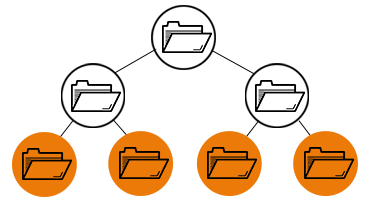
\includegraphics{Pictures/FileStorageHierarchy.png}
	\caption{File Storage: Aufbau des Hierarchiesystems, \citeauthor{redHat-storage}}
\end{figure}

File Storage wird häufig in Unternehmen und Organisationen eingesetzt, um gemeinsame Dateiserver bereitzustellen oder Daten in Cloud-Speicherdiensten wie Dropbox oder Google Drive zu speichern.
Auch wenn es von Betriebssystemen und Anwendungen gut unterstützt wird, kann die Performance und Skalierbarkeit von File Storage bei sehr großen Dateisystemen beeinträchtigt werden, was insbesondere bei stark frequentierten Anwendungen oder bei der Verarbeitung großer Datenmengen zum Problem werden kann. 

\begin{quote}
	Mit zunehmenden Datenvolumen erfordert das Skalieren von Dateispeichern das Hinzufügen neuer Hardwaregeräte oder den Austausch vorhandener Geräte durch solche mit höherer Kapazität. Dies kann im Laufe der Zeit teuer werden. \glqq As data volumes expand, scaling file storage requires [...]\grqq, (\cite{nx-fileScala}, Übersetzung des Autors)
\end{quote}

Laut Wahlmann (\citeyear{nx-fileScala}, Übersetzung des Autors) wird die Datenspeicherung bei zu vielen Daten nicht nur teuer, sondern auch unhandlich und zeitaufwändig. Der schnelle und einfache Zugriff auf jede einzelne Datei wird schwierig, wenn man zig Millionen von Dateien in Tausenden von Verzeichnissen auf Hunderten von Speichergrößen speichert. 

\subsection{Block Storage}

Block Storage, auch genannt als Block-level Storage speichert Dateien auf SAN(Storage Area Networks) basierten Netzwerken oder auf Cloud-basierten Speicherumgebungen. Das System teilt Daten in Blöcke auf und speichert die separaten Teile jeweils mit einer eindeutigen Kennung, vgl. \cite{ibm-topics}.\\

Daten werden in Blöcken auf dem Datenträger gespeichert, die unabhängig voneinander adressiert werden können. Jeder Block ist eine feste Größe, typischerweise im Bereich von einigen Kilobytes bis hin zu einigen Megabytes. Diese Blöcke können im System an jeder Stelle gespeichert werden.

\begin{quote}
	Wenn auf Block Storage gespeicherte Daten abgerufen werden, verwendet das Server-Betriebssystem die eindeutige Adresse, um die Blöcke wieder zusammenzufügen und so die Datei zu erstellen. Der Vorteil besteht darin, dass das System nicht durch Verzeichnisse und Dateihierarchien navigieren muss, um auf die Datenblöcke zuzugreifen. Dadurch werden Effizienzen erzielt, da der Abruf von Daten schneller erfolgen kann, vgl. \cite{ibm-storage}.
\end{quote}

Typische Anwendungsbereiche des Block Storage sind Datenbanken, Virtualisierungsumgebungen und Anwendungen für Big Data-Analysen. Speicherung von strukturierten Daten wie Datenbanken, Virtuelle Maschinen und Betriebssysteme eignen sich besonders bei der Verwendung von Block Storage. Diese Art von Daten erfordert schnellen und direkten Zugriff auf bestimmte Bereiche des Speichers und muss häufig in Echtzeit ausgeführt werden. Block Storage eignet sich daher am besten für Anwendungen mit hohen Anforderungen an die Leistung und niedriger Latenzzeit.

\newpage

\subsection{Object Storage}

Object Storage hat sich als Speichertechnologie in den letzten Jahren immer stärker etabliert und wird von vielen Unternehmen als Alternative zu traditionellen Speicherlösungen wie Block- oder File Storage angesehen. Die ersten Object Storage Systeme wurden bereits in den 1990er Jahren entwickelt, aber erst mit dem Aufkommen von Big Data, IoT und der Cloud-Nutzung 
 hat es einen breiteren Einsatz gefunden. Heute bieten viele Cloud Provider wie Amazon Web Services (AWS) und Google Cloud Platform (GCP) Object Storage als einen ihrer Haupt-Cloud-Services an.\\
 
\begin{quote}
	Object Storage ist für den Umgang mit großen Datenvolumen und unstrukturierten Daten entwickelt wurden. Sie speichert Daten als eigenständige Objekte, die aus Daten und Metadaten bestehen und einen eindeutigen Identifier (UID) haben (\glqq Object storage (aka object-based storage) is a type of data storage used to [...]\grqq, \cite{dataCore-OS}, Übersetzung des Autors).
\end{quote}

Im Gegensatz zu hierarchischen Systemen wie beim File Storage ist das Speichersystem flach strukturiert. Durch die einfache API Anbindung kann es mit vorhandenen Anwendungen integriert werden. Nutzer können detaillierte Informationen wie beispielsweise Erstellerangaben, Schlüsselwörter sowie Sicherheit-und Datenschutzrichtlinien hinterlegen. Diese Daten bezeichnet man als Metadaten.\\

Laut \citeauthor{nx-fileScala}, 2022 ist Skalierbarkeit der Hauptvorteil, da bei der Speicherung von Petabyte und Exabyte alle Objekte in einem Namespace abgelegt werden. Selbst wenn dieser Namespace auf Hunderte von Hardwaregeräten und Standorten verteilt ist, können alle Objekte schnell abgerufen werden. Andere Vorteile von Objekt Storage beinhalten die Datenintegritätsprüfung, im Englischen bekannt als \glqq erasure coding\grqq und die Datenanalyse.\\

Auch Object Storage hat seine Nachteile. Laut \citeauthor{redHat-storage} muss das Objekt nach der Speicherung bei Veränderung komplett neu überschrieben werden. Sie sind für traditionelle Datenbanken nicht geeignet, da das Schreiben von Objekten Zeit beansprucht und man sich mit der API auseinandersetzen muss, vgl. \citeauthor{redHat-storage}.\\

Insgesamt bietet Object Storage eine skalierbare und flexible Methode zur Speicherung von unstrukturierten Daten. Organisationen sollten jedoch die Vor- und Nachteile von Object Storage im Kontext ihrer spezifischen Anwendungsfälle abwägen, um eine fundierte Entscheidung über die beste Speichermethode zu treffen.\\

%TODO Object Storage Entscheidung

Da leoticket Daten wie Rechnungen und Tickets als Dateien speichern und abrufen abruft, ist Object Storage die richtige Speicherart. 

Für leoticket ist die Object Storage Variante die am Besten geeignetste Speicherlösung, da ... %TODO Satz weiterschreiben


\section{Aktuelle Speichertechnologien im Markt}

Die beiden größten Cloud-Speicheranbieter, Amazon Web Services (AWS) und Google Cloud Platform (GCP), bieten eine Vielzahl von Speicherlösungen an, die auf die Bedürfnisse von Unternehmen zugeschnitten sind.\\ 

In diesem Kapitel werden die aktuellen Speichertechnologien auf dem Markt untersucht, wobei der Fokus auf den Angeboten von AWS und GCP liegt. Um eine Vergleichsgrundlage zwischen AWS und GCP zu schaffen, werden die verschiedenen Aspekte wie sichere Speicherung, Hochverfügbarkeit, Leistung, Kosten, API Anbindung und die Bereitstellung der Dateien betrachtet. Dieses Vorgehen dient dazu, zu ermitteln, welche Speicherart sich am besten für welche Anforderungen eignet. Als Kontrast dazu wird das Open-Source-Objektspeichersystem MinIO betrachtet.\\

AWS bietet eine Reihe von Speicheroptionen an, darunter Amazon S3 (Simple Storage Service). Amazon S3 ist ein Object Storage-Service, der für die Speicherung und den schnellen Abruf von unstrukturierten Daten wie Videos, Fotos und Dokumenten ausgelegt ist.

Google Cloud Platform bietet ebenfalls eine Vielzahl von Speicherlösungen an, darunter Google Cloud Storage. Google Cloud Storage ist ein Object Storage-Service, der für die Speicherung von unstrukturierten Daten wie Bildern, Videos und Dokumenten ausgelegt ist.\\
 
Insgesamt bieten AWS und Google Cloud Platform eine Vielzahl von Speicherlösungen an, die auf die Bedürfnisse von Unternehmen zugeschnitten sind. Organisationen sollten jedoch die Vor- und Nachteile jeder Speicherlösung abwägen, um die beste Lösung für ihre spezifischen Anforderungen zu finden.

\newpage

\subsection{Eigenschaften}

Im vorliegenden Abschnitt werden Amazon S3 und Google Cloud Storage in Bezug auf verschiedene Kriterien untersucht. Dabei werden zunächst die Eigenschaften von AWS S3 erläutert, gefolgt von einer Betrachtung von GC Storage. Ziel ist es, die Unterschiede zwischen den beiden Anbietern hervorzuheben und eine Entscheidungshilfe zu bieten, welche Plattform für die Anforderungen von \glqq leoticket\grqq am besten geeignet ist. Die Auswahl der Kriterien erfolgt in Anlehnung an die spezifischen Anforderungen von \glqq leoticket\grqq.

%TODO Aws und GCP Definition?

\subsubsection{Sichere Speicherung}

\textbf{AWS S3}\\

Viele Anbieter von Object Storage-Lösungen bieten integrierte Verschlüsselungsmöglichkeiten an, um sicherzustellen, dass Daten sowohl in Ruhe als auch in Bewegung geschützt sind. Dabei können unterschiedliche Verschlüsselungsmethoden zum Einsatz kommen.In Bezug auf die sichere Speicherung bieten sowohl AWS als auch GCP verschiedene Optionen für die Verschlüsselung von Daten.\\



AWS bietet beispielsweise den Server-Side-Encryption (SSE) mit AWS-Managed-Keys und SSE mit KMS-Managed-Keys an, während GCP Server-Side-Encryption with Customer-Supplied Encryption Keys (CSEK) sowie Server-Side-Encryption with Google-managed encryption keys (SSE) anbietet. Beide Cloud-Anbieter bieten auch die Möglichkeit der Client-seitigen Verschlüsselung. In Bezug auf Datenschutzstandards hat AWS die ISO/IEC 27001-, 27017- und 27018-Zertifizierungen erhalten, während GCP die ISO/IEC 27001-, 27017-, 27018- und 27701-Zertifizierungen erhalten hat.


\subsubsection{Hochverfügbarkeit}
\subsubsection{Performance}
\subsubsection{Kosten}
\subsubsection{API Anbindung}

\subsection{Bereitstellung der Dateien}

\section{Auswahl des Speichersystems}

In diesem Abschnitt wird durch eine Kosten-, und Performance Analyse die Speichersysteme ausgewertet und eine Auswahl getroffen. Die Kalkulationsergebnisse werden zum Schluss dargestellt.

\subsection{Kostenanalyse}
\subsection{Performance Analyse}
\subsection{Kalkulationsergebnisse}